\documentclass{article}
\usepackage[margin=1.0in]{geometry}
\usepackage{amsmath, amssymb, mathrsfs}
\usepackage[english]{babel}
\usepackage{graphicx}
\usepackage{enumerate}
\usepackage{listings}
\usepackage{pgfplots}
\usepackage{tikz}
\renewcommand{\vec}[1]{\mathbf{#1}}
\newcommand{\floor}[1]{\left\lfloor #1 \right\rfloor}
\newcommand{\ceil}[1]{\left\lceil #1 \right\rceil}

\title{Machine Learning from Data Assignment 5}
\author{Greg Stewart}
\date{\today}

\begin{document}

\maketitle

\subsection*{Exercise 2.8}

\begin{enumerate}[(a)]
  \item \textit{Show that if $H$ is closed under linear combination, then $\overline{g} \in H$.}

    The definition of of $\overline{g}(x)$ is 
      
      $$\overline{g}(x) = \frac{1}{K}\sum_{k=1}^{K} g_k(x).$$

    This means that every value of $\overline{g}$ is a multiple of of the values of $g$ in $H$.
    In other words, it is a linear combination of the $g_k \in H$. Since $H$ is closed under
    linear combination, $\overline{g}$ must also be in $H$.

  \item \textit{Give a model for which the average function $\overline{g}$ is not in the model's
    hypothesis set.}

    If $H = \emptyset$, then $\overline{g}$ cannot be in $H$.

  \item \textit{For binary classification, do you expect $\overline{g}$ to be a binary function?}

    No, this is unlikely.

\end{enumerate}



\subsection*{Problem 2.14}

\textit{Let $H_1, H_2, \dots, H_K$ be $K$ hypothesis sets with finite VC dimension $d_{VC}$.
Let $H = H_1 \cup H_2 \cup \cdots \cup H_K$ be the union of these models.}

\begin{enumerate}[(a)]
  \item \textit{Show that $d_{VC}(H) < K(d_{VC} + 1)$.}

    The hypothesis sets have VC dimension $d_{VC}$, meaning they have break point 
    $k^* = d_{VC}+1$. Recall that the first break point is the sample size for which not all
    dichotomies can be given by the hypothesis set. So, given $K$ hypothesis sets with this break
    point, if every hypothesis set can fill out dichotomies that others can't we end up with
    a largest possible breakpoint of $$k^*(H) = Kk^*.$$ Since the breakpoint is related to the VC
    dimension and this is the largest value, we can rewrite this as

    $$d_{VC}(H) < K(d_{VC}+1)$$

    since the VC dimension is strictly less than $k*$.


  \item \textit{Suppose that $l$ satisfies $2^l > 2Kl^{d_{VC}}$. Show that $d_{VC}(H) \leq l$.}

    This is a straight proof by calculation.

    \begin{align*}
      2^l &> 2Kl^{d_{VC}} \\
      2^{l-1} &> Kl^{d_{VC}} \\
      (l-1)\log_2 2 &> K d_{VC} \log_2 l \\
      d_{VC} &< (l-1) \frac{1}{K \log_2 l}\\
      &\leq \frac{l-1}{K} \\
    \end{align*}

    And as we can add this together $K$ times for $d_{VC}(H)$, we get

    $$d_{VC}(H) \leq K \frac{l-1}{K} = l-1$$

    which implies $$d_{VC}(H) \leq l.$$

  \item \textit{Hence, show that
    $$d_{VC}(H) \leq \min(K(d_{VC}+1), 7(d_{VC}+K)\log_2(d_{VC}K)).$$
    That is, $d_{VC} = O(\max(d_{VC},K)\log_2\max(d_{VC},K))$ is not too bad.}

    Obviously, if the bound from (a) is the lower of the two, the inequality above holds.

    To show the second term in the min is a bound, we set $l$ to it and substitute into the
    inequality from (b).

    \begin{align*}
      2^{7(d_{VC}+K)\log_2(d_{VC}K)} &> 2K(7(d_{VC}+K)\log_2(d_{VC}K))^{d_{VC}} \\
      (d_{VC}K)^{7(d_{VC}+K)} &> 2K(7(d_{VC}+K)d_{VC}\log_2(d_{VC}K)) \\
      (d_{VC}K)^{7(d_{VC}+K)-1} &> 2(7(d_{VC}+K)\log_2(d_{VC}K)) \\
    \end{align*}

    This inequality, ugly as it is, holds for $K > 1$, so we have shown the previous inequality
    is true.


\end{enumerate}

\subsection*{Problem 2.15}

\textit{The monotonically increasing hypothesis set is
$$H = \{h \mid x_1 \geq x_2 \implies h(x_1) \geq h(x_2)\},$$ where $x_1\geq x_2$ if and only if
the inequality is satisfied for every component.}

\begin{enumerate}[(a)]
  \item \textit{Give an example of a monotonic classifier in two dimensions, clearly showing
    the +1 and -1 regions.}

    The monotonic classifier will appear as a sort of decreasing step function, with the upper
    right side being the +1 region and the -1 region being the bottom left side.

    \begin{center}
      \begin{tikzpicture}
      \begin{axis}[%
          ,ymax=1.1 % or enlarge y limits=upper
          ,ymin=0.0
          ,xmin=0.0
          ,yticklabels={,,}
          ,xticklabels={,,}
          ]
        %\addplot+[const plot, no marks, thick] coordinates {(0,1) (1,0.7) (2,0.5) (3,0.3) (4,0)} node[above,pos=.4,black] {$-$} node[above,pos=.525,black]{$+$};
        \addplot+[const plot, no marks] coordinates {(0,1) (1,0.7) (2,0.5) (3,0.3) (4,0)} node[above,pos=.4,black] {$-$} node[above,pos=.525,black]{$+$};
      \end{axis}
      \end{tikzpicture}
    \end{center}

  \item \textit{Compute $m_H(N)$ and hence the VC dimension.}

    Consider the case of $N$ monotonically decreasing points in the Cartesian plane. With the
    monotonically increasing hypothesis set, \textbf{all dichotomies are possible}. Thus,

    $$m_H(N) = 2^n \qquad \text{and} \qquad d_{VC} = \infty.$$

\end{enumerate}



\subsection*{Problem 2.24}

\textit{Assume input dimension 1. Assume input variable $x$ is uniformly distributed in the
interval [-1,1]. Data set consists of 2 points, $\{x_1,x_2\}$. Assume target function is 
$f(x) = x^2$. Full data set is $D = \{ (x_1, x_1^2), (x_2, x_2^2) \}$. Learning algorithm
returns line fitting these two points as $g$. We are interested in the test performance $E_{out}$
of the learning system w.r.t. the squared error measure, the bias and the variance.}

\begin{enumerate}[(a)]
  \item \textit{Give the analytic expression for the average function $\overline{g}(x)$.}

    $$\overline{g}(x) \approx \frac{1}{K}\sum_{k=1}^K g_k(x) = \mathbb{E}[ax+b]$$

    $a$ is the slope of the line obtained from the points, and $b$ the intercept, so we get

    \begin{align*}
      \overline{g}(x) &= \mathbb{E}[(x_1 + x_2)x - x_1x_2] \\
      &= \mathbb{E}[x_1] + \mathbb{E}[x_2])x - \mathbb{E}[x_1]\mathbb{E}[x_2] \\
      &= 0
    \end{align*}

  \item \textit{Describe an experiment that you could run to determine numerically 
    $\overline{g}(x), E_{out}$, bias, and var.}

    Generate a large number (e.g. 10,000) of 2-point datasets 
    $D = \{ (x_1, x_1^2), (x_2, x_2^2) \}$ and generate the set of final hypotheses for all these
    data sets. Since each $g_i$ is just a line, we can simply store the coefficients $a,b$ of 
    $g = ax + b$, then average the sets of each coefficient to obtain $\overline{g}(x)$. The
    typical formula for $E_{out}$ can be used for each iteration, then averaged. Bias and
    variance can both be calculated using $\overline{g}$.


  \item \textit{Run your experiment and report the results. Compare $E_{out}$ with bias+var.
    Provide a plot of your $\overline{g}(x)$ and $f(x)$.}

    Running the experiment for $N = 10000$ gives

    \begin{align*}
      \overline{g}(x) &= 0.00244 x + 0.00143 \\
      E_{out} &= 0.537 \\
      \mathbb{E}[bias(x)] &= 0.204 \\
      \mathbb{E}[var(x)] &= 0.331 \\
    \end{align*}
    
    So for $bias + var$ we get 0.535, only two thousands from the value first obtained for
    $E_{out}$. These values are extremely close, exactly as expected.

    \begin{center}
    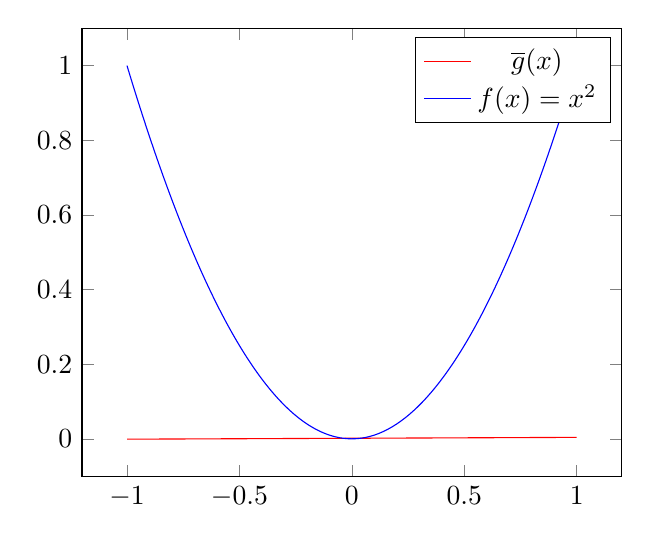
\begin{tikzpicture}
      \begin{axis}
        \addplot [
          domain = -1:1,
          samples = 1000,
          color = red,
        ] {0.00244*x + 0.00143};
        \addlegendentry{$\overline{g}(x)$}
        \addplot [ 
          domain = -1:1,
          samples = 1000,
          color = blue,
        ] {x^2};
        \addlegendentry{$f(x) = x^2$}
      \end{axis}
    \end{tikzpicture}
    \end{center}

  \item \textit{Compute analytically what $E_{out}$, bias, and var should be.}

    For bias we have

    \begin{align*}
      bias &= \mathbb{E}_x[\overline{g}(x) - f(x))^2] \\
      &= \frac{1}{2}\int_{-1}^1 x^4 dx \\
      &= \frac{1}{5}
    \end{align*}

    and for variance we get 

    \begin{align*}
      var &= \mathbb{E}_x[\mathbb{E}_D[(g_D(X) - \overline{g}(x))^2]] \\
      &= \frac{1}{4}\int_{-1}^1\int_{-1,1}\int_{-1}^1 ((y+z)x-yz)^2 dy dz dx \\
      &= \frac{1}{3}
    \end{align*}

    so for $E_{out}$ we get

    \begin{align*}
      \mathbb{E}[E_{out}] &= bias + var \\
      &= \frac{1}{5} + \frac{1}{3} \\
      &= \frac{8}{15} \approx .533
    \end{align*}

    All of these values agree well with the numerically obtained values.














\end{enumerate}



\end{document}
